\section{Theorie}
\label{sec:Theorie}

Als Ultraschall wird der Schall bezeichnet, welcher in dem Frequenzbereich oberhalb der von Menschen hörbaren Frequenzen liegt.
Dieser Bereich liegt etwa zwischen $\SI{20}{\kilo\hertz}$ und $\SI{1}{\giga\hertz}$.
Dieser Schall kann dazu verwendet werden Materialien auf Fehlstellen zu untersuchen, ohne dieses zu zerstören.

Hierbei gibt es zwei verschiedene Untersuchungsverfahren.
Das Durchschallungsverfahren sendet einen Schallimpuls durch ein Medium und dieser Impuls wird auf der anderen Seite empfangen und auf Zeitdifferenz und Amplitudendifferenz untersucht.
Beim Impuls-Echo-Verfahren wird der ausgesendete Impuls an einer Grenzfläche reflektiert und dieser reflektierte Impuls wird untersucht.

Letzteres Verfahren kann auch dazu verwendet werden die Fließgeschwindigkeit einer Objekten in einer Flüssigkeit zu untersuchen.
In der Medizin werden so z.B. Blutströmungen untersucht.
Dafür wird der Doppler-Effekt genutzt, welcher auch der Namensgeber für die hier beschriebene Doppler-Sonographie ist.
Dieser besagt, dass die Bewegung einer Quelle von Schallwellen die Frequenz der Schallwelle beeinflusst.
Nähert sich die Quelle dem Betrachter, so wird die Frequenz zu einer höheren Frequenz verschoben und entfernt sich die Quelle, so wird die Frequenz zu einer niedrigeren Frequenz verschoben.
Die neue Frequenz kann über
\begin{equation}
    \nu = \frac{\nu_0}{1 \pm \frac{v}{c}}
    \label{eq:frequenz_quellenbewegung}
\end{equation}
berechnet werden, wobei $\nu_0$ die Frequenz der erzeugten Schallwelle, $v$ die relative Geschwindigkeit der Quelle zum Beobachter und $c$ die Schallgeschwindigkeit des Mediums ist.

Der Effekt funktioniert analog, wenn man sich im Inertialsystem der Quelle befindet. 
Hier lässt sich die beobachtete Frequenz über
\begin{equation}
    \nu = \nu_0 \left( 1 \pm \frac{v}{c} \right)
    \label{eq:frequenz_beobachterbewegung}
\end{equation}
berechnen.

\begin{figure}
    \centering
    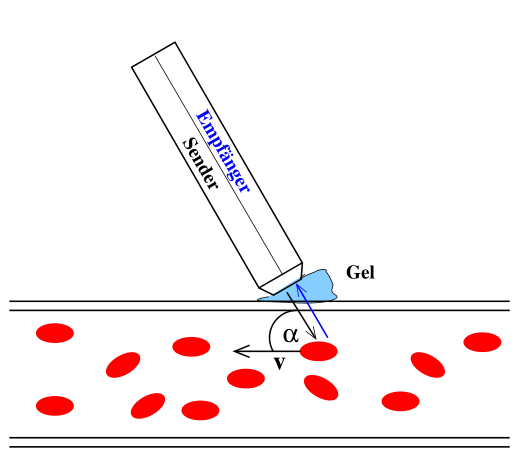
\includegraphics[width=0.3\textwidth]{images/skizze_1.png}
    \caption{Schema des Impuls-Echo-Verfahrens bzw. der Doppler-Sonographie \cite{US3}}
    \label{fig:skizze_alpha}
\end{figure}

Da beim Impuls-Echo-Verfahren der Schallimpuls nicht parallel zur Fließrichtung ausgesendet und empfangen wird, muss der Winkel $\alpha$ beachtet werden. (siehe \autoref{fig:skizze_alpha})
Somit kann die Frequenzverschiebung über
\begin{equation}
    \Delta \nu = 2 \nu_0 \frac{v}{c} \cos \alpha
    \label{eq:Frequenzverschiebung}
\end{equation}
berechnet werden.
Umstellen dieser Gleichung führt zu einer Berechnungsformel für die Fließgeschwindigkeit
\begin{equation}
    v = \frac{\Delta \nu \cdot c}{2 \cdot \nu_0 \cdot \cos \alpha}
    \label{eq:geschwindigkeit}
\end{equation}

Als Quelle und Empfänger wird in diesem Versuch ein sogenannter piezo-elektrischer Kristall verwendet.
Wird an diesem ein elektrisches Feld entlang seiner polaren Achse angelegt kontrahiert bzw. expandiert er.
So können Schallwellen mit einer hohen Frequenz erzeugt werden.
Wenn die Frequenz im Resonanzbereich des Kristallsliegt kann auch ein Schallwelle mit genügend hoher Amplitude erzeugt werden.
Andersherum erzeugt der Kristall ein elektrisches Feld wenn auf diesen Schallwellen treffen.
Also kann der Kristall sowohl als Sender als auch als Empfänger verwendet werden.